% !TeX spellcheck = en_US
\addsection{Difficulty}{\spells/berserk.png}

\begin{multicols}{2}

During setup, players must choose the game's \hypertarget{Difficulty}{Difficulty}\index{Difficulty}.
There are four different Difficulties, each with a different starting bonus\index{Starting Bonus} that players receive during step 16 of the setup:
\begin{itemize}
  \item \textbf{Easy} – Roll 2 \includesvg[height=10px]{\svgs/resource_die.svg} and receive Resources from both – OR – \textbf{Search} (2) the Artifact Deck, twice.
  \item \textbf{Normal} – Roll 2 \includesvg[height=10px]{\svgs/resource_die.svg} and receive the Resources from one of them – OR – \textbf{Search} (2) the Artifact Deck.
  \item \textbf{Hard} – Roll 1 \includesvg[height=10px]{\svgs/resource_die.svg} and receive the Resources on it – OR – reveal cards from the top of the Artifact Deck until you find 1 Minor Artifact and add it to your hand.
  \item \textbf{Impossible} – No starting bonus.
\end{itemize}

\columnbreak

Campaign missions have unique bonuses that \textbf{replace} the regular starting bonus.

All \textbf{Artifacts} received from a starting bonus should be placed into your \textbf{hand} and not shuffled into your Starting Deck.
If you searched for any Artifacts, shuffle the Artifact Deck and its Discard Pile\index{Discard Pile} together afterwards, and then discard one Artifact from the top to form the Artifact Discard Pile again.\par
The chosen difficulty also determines the number and type of neutral enemies that are encountered during Neutral Combat according to the \hyperlink{Difficulty Table}{table} at the back cover of the book.

\end{multicols}

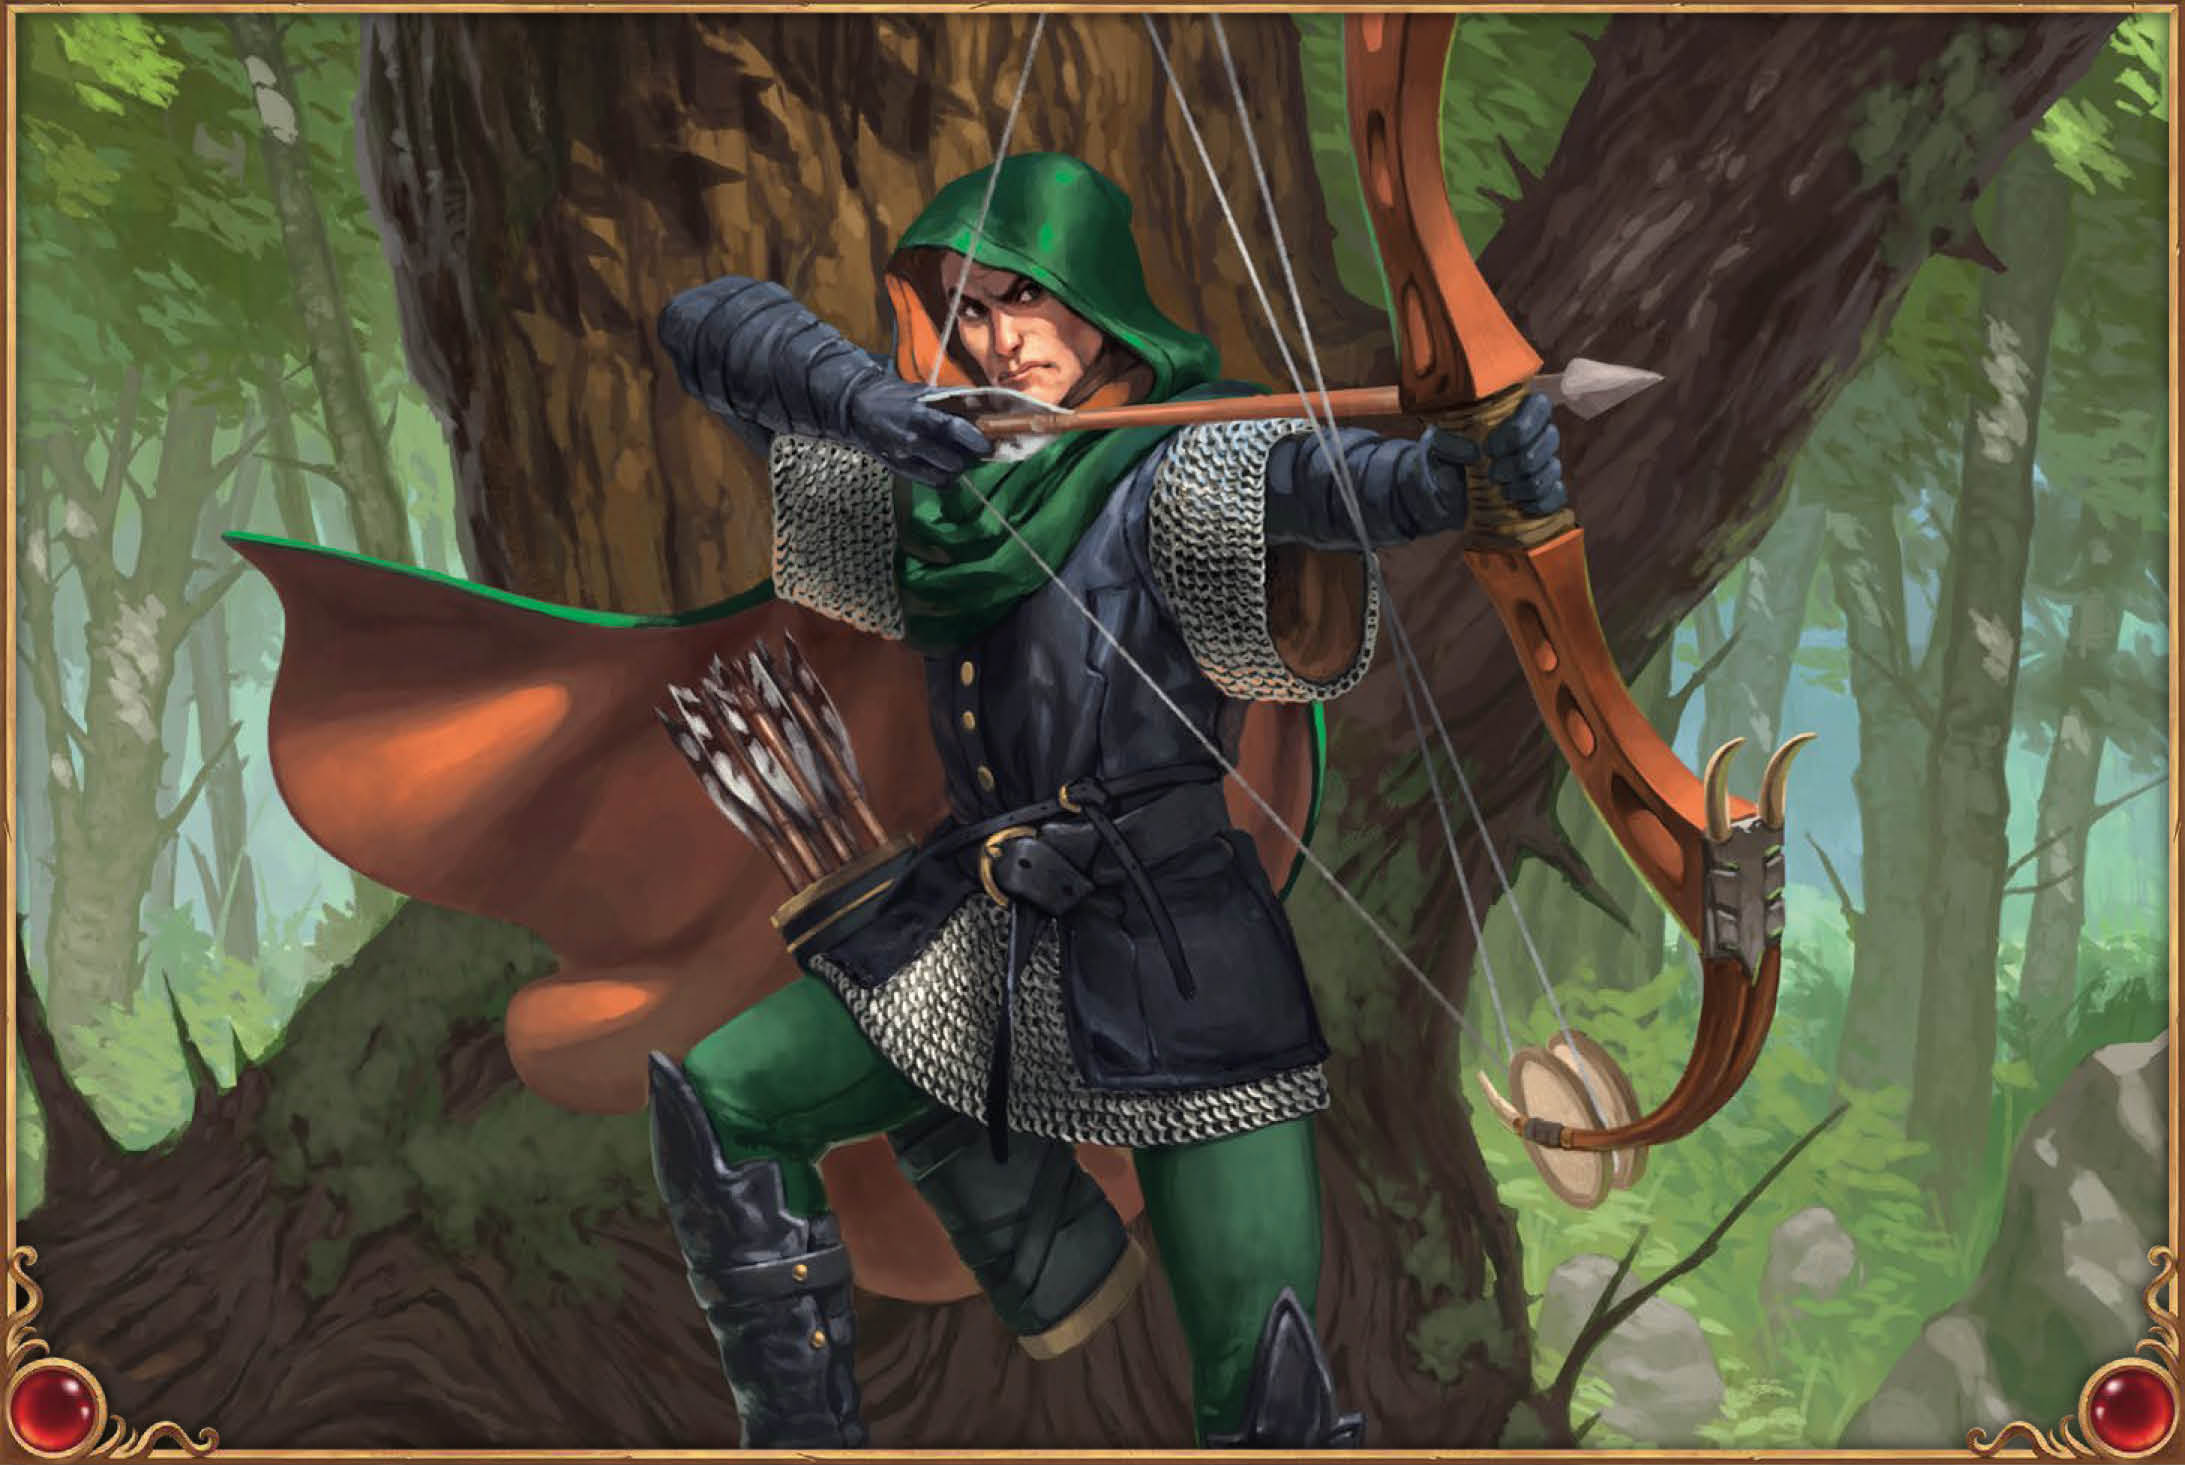
\includegraphics[width=\linewidth]{\art/sharpshooter.jpg}

\clearpage

\vspace*{-3em}
\hommtable{38}{
  \centering
  \textbf{Optional Rules Table}

  \small
  {
    \color{white}
    You may modify the rules to increase or decrease the game's difficulty.
  }
  \bigskip

  \begin{tabularx}{\linewidth}{>{\hsize=0.3\hsize\linewidth=\hsize}X
                               >{\hsize=1.7\hsize\linewidth=\hsize}X}
     \darkcell[1.5]{\color{white}Game Difficulty Levels} & \darkcell[1.5]{Change to the default rules} \\
     \darkcell[1.2]{Increase} & \lightcell[1.2]{Towns do not produce resources when \textbf{Flagged}, but players may use the buildings of a captured Town.} \\
     \darkcell[0.8]{Increase} & \lightcell[0.8]{You may not reroll your dice.} \\
     \darkcell[0.8]{Increase} & \lightcell[0.8]{All Treasure and Resource dice only give 1 resource.} \\
     \darkcell[0.8]{Increase} & \lightcell[0.8]{No starting bonus.} \\
     \darkcell[0.8]{Decrease} & \lightcell[0.8]{You start the game with a Secondary Hero.} \\
     \darkcell[0.8]{Decrease} & \lightcell[0.8]{Every unit deal at least 1 \includesvg[height=10px]{\svgs/damage-table.svg} during an attack.} \\
     \darkcell[0.8]{Decrease} & \lightcell[0.8]{All Mines and Settlements provide double income.} \\
     \darkcell[1.2]{Decrease} & \lightcell[1.2]{You may exchange your resources at any time, the Trading Post becomes \textbf{Visitable} and draws you 1 card from the Artifact deck.} \\
     \darkcell[0.8]{Decrease} & \lightcell[0.8]{Extending Combat no longer costs any MP.} \\
     \darkcell[0.8]{Variant} & \lightcell[0.8]{The Attack die no longer affects damage (but can still interact with abilities).} \\
     \darkcell[0.8]{Variant} & \lightcell[0.8]{An Astrologers Proclaim card is also drawn at the start of the Resource rounds.} \\
     \darkcell[0.8]{Variant} & \lightcell[0.8]{Astrologers Proclaim cards are no longer drawn.} \\
     \darkcell[0.8]{Variant} & \lightcell[0.8]{Black cubes on all \textbf{Visitable} fields are removed on \nth{4}, \nth{8}, and \nth{12} rounds.} \\
     \darkcell[1.2]{Variant} & \lightcell[1.2]{The cards that would normally go to your hand now go immediately to your discard pile instead.} \\
  \end{tabularx}
}

\vspace*{-1em}

\framedimage[\linewidth]{\art/devil.jpg}
